The project will consist of two separate development efforts, consisting of a hosted application to source and correlate data and a mobile application to display events and report disruptions. In order to describe the system, the requirements were identified with goal-oriented capture\cite{Requirements}.

\begin{figure}[here]
\begin{center}
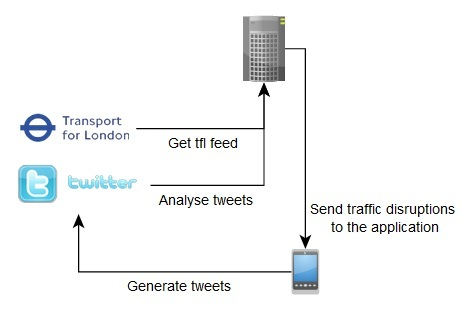
\includegraphics[width=0.5\textwidth]{images/draft_architecture.jpg}
\end{center}
\vspace{-20pt}
\caption{Application Architecture}
\end{figure}

The hosted application will retrieve traffic events from a Transport for London (TfL) data feed and correlate each event with relevant tweets harvested from Twitter. The server based application gathers data from TfL and Twitter periodically. TfL provides a curated feed of ongoing traffic disruptions in a structured format. Twitter provides us with a torrent of unsorted tweets, from which relevant tweets must be extracted. In addition traffic disruptions reported from the mobile application can be identified through the use of a hash tag, enabling these messages to be processed separately. The server gathers the TfL data and then tries to match tweets about these traffic disruptions. To discover tweets that discuss traffic concepts, document classification techniques must be utilised. Two points we can improve on the server is the classification algorithm, and adding the functionality to generate traffic disruptions that are reported only from Twitter, and not yet on TfL.

The mobile application must provide the commuter with a mechanism for discovering disruptions that may affect their route. This is to be provided through the use of a map based interface. In addition the mobile application must offer the user the ability to comment or describe an on going traffic disruption. The user interface for reporting disruptions must offer a quick and intuitive mechanism for describing a particular event, while also satisfying users that require more control over the messages published on their account.

Below there are tables for every feature and its priority, feasibility and expected completion date. The smaller number in priority means more important to finish fast (1-10) and in feasibility the smaller number means more achievable (1-10).

\begin{center}
\begin{tabular}{ | p{6cm} | c | c | c | }
\hline
\multicolumn{4}{|c|}{\textbf{Mobile Application}} \\ \hline
\textbf{Feature} & \textbf{Priority} & \textbf{Feasibility} & \textbf{Expected completion} \\ \hline
\textbf{Report events}\newline
Report traffic disruption through the mobile application on Twitter, using a hash tag. & 1 & 2 & \\ \hline
\textbf{Present a list of classified and grouped tweets}\newline
Present to the user tweets identified as describing a traffic disruption,
clustered around an event. & 2 & 4 & \\ \hline
\textbf{Show local disruption map}\newline
Show positions of known disruptions on a map. Enabling the user to click on a
particular event for further information. & 3 & 5 & \\ \hline
\textbf{Stored Routes}\newline
Find and show disruptions for user defined stored routes. & 4 & 7 & \\ \hline
\end{tabular}
\end{center}
Minimum specifications for the mobile application are all features including
and below priority 3.
\begin{center}
\begin{tabular}{ | p{6cm} | c | c | c | }
\hline
\multicolumn{4}{|c|}{\textbf{Server Hosted Application}} \\ \hline
\textbf{Feature} & \textbf{Priority} & \textbf{Feasibility} & \textbf{Expected completion} \\ \hline
\textbf{Store disruptions from TfL} \newline
Create a geographic database of live events from TfL. Evolve these database events with data from the feed, in order to have a current representation of the event. & 1 & 3 & \\ \hline
\textbf{Store and categorise social data} \newline
For tweets with an explicit location store these in a geographical database
table. And for tweets without this explicit information store for later
analysis. & 2 & 2 & \\ \hline
\textbf{Process mobile client reports} \newline
Take twitter messages reported from the mobile client and process these in a
separate pipeline. & 3 & 2 & \\ \hline
\textbf{Identify traffic disruptions from Twitter} \newline
Analyse incoming traffic tweets and determine new non-TfL disruptions from
those. & 4 & 5 & \\ \hline
\textbf{Classify tweets from Twitter with a simple classifier} \newline
Identify traffic related tweets with a simple classifier and store those
tweets, using their geographic representation as a key. & 5 & 5 & \\ \hline
\textbf{Geocoding of messages without explicit locations} \newline
Resolve geographic locations extracted from the message context. & 6 & 7 & \\ \hline
\textbf{Enhance classification and clustering algorithms} \newline
From insight and data gained from initial classification and clustering
techniques, attempt to improve the accuracy of the results. & 7 & 9 & \\ \hline
\end{tabular}
\end{center}
Minimum specifications for the server application are all features including
and below priority 4.
